%%%%%%%%%%%%%%%%%%%%%%%%%%%%%%%%%%%%%%%%%%%%%%%%%%%%%%%%%%%%%%%%%%%%%%%%%%%%%%%%
%2345678901234567890123456789012345678901234567890123456789012345678901234567890
%        1         2         3         4         5         6         7         8

\documentclass[letterpaper, 10 pt, conference, onecolumn]{ieeeconf}  % Comment this line out
                                                          % if you need a4paper
%\documentclass[a4paper, 10pt, conference]{ieeeconf}      % Use this line for a4
                                                          % paper

\IEEEoverridecommandlockouts                              % This command is only
                                                          % needed if you want to
                                                          % use the \thanks command
\overrideIEEEmargins
% See the \addtolength command later in the file to balance the column lengths
% on the last page of the document



% The following packages can be found on http:\\www.ctan.org
\usepackage{graphics} % for pdf, bitmapped graphics files
\usepackage{epsfig} % for postscript graphics files
\usepackage{mathptmx} % assumes new font selection scheme installed
\usepackage{times} % assumes new font selection scheme installed
\usepackage{amsmath} % assumes amsmath package installed
\usepackage{amssymb}  % assumes amsmath package installed
%\usepackage{cleveref}
\usepackage{tabularx}
\usepackage{adjustbox}
\usepackage{hyperref}

\hypersetup{
    %pagebackref=true,
	pdftitle={Predicting remaining useful life of aircrafts' turofan engines}, 
	pdfauthor={Fernando Martinelli Ramacciotti},
	%pdfkeywords={abnt}{latex}{abntex}{abntex2}{trabalho acadêmico}, 
	colorlinks=true,       		% false: boxed links; true: colored links
    linkcolor=blue,          	% color of internal links
    citecolor=black,        		% color of links to bibliography
    %filecolor=magenta,      		% color of file links
	urlcolor=blue,
	bookmarksdepth=4
}

\title{\LARGE \bf
Predicting remaining useful life of aircrafts' turofan engines}

%\author{ \parbox{3 in}{\centering Huibert Kwakernaak*
%         \thanks{*Use the $\backslash$thanks command to put information here}\\
%         Faculty of Electrical Engineering, Mathematics and Computer Science\\
%         University of Twente\\
%         7500 AE Enschede, The Netherlands\\
%         {\tt\small h.kwakernaak@autsubmit.com}}
%         \hspace*{ 0.5 in}
%         \parbox{3 in}{ \centering Pradeep Misra**
%         \thanks{**The footnote marks may be inserted manually}\\
%        Department of Electrical Engineering \\
%         Wright State University\\
%         Dayton, OH 45435, USA\\
%         {\tt\small pmisra@cs.wright.edu}}
%}

\author{Fernando Martinelli Ramacciotti \\ 
fernandoramacciotti@gmail.com% <-this % stops a space
}


\begin{document}



\maketitle
\thispagestyle{plain}
\pagestyle{plain}


%%%%%%%%%%%%%%%%%%%%%%%%%%%%%%%%%%%%%%%%%%%%%%%%%%%%%%%%%%%%%%%%%%%%%%%%%%%%%%%%
\begin{abstract}

\textbf{
Predicitve maintenance through predicting remaining useful life (RUL) of an asset is desired for every business. Data-driven approaches can yield good results, but such data is costly to collect, once companies would lose money to run their machines to failure. NASA has simulated several run-to-failure conditions for a fleet of turbofan engines and such dataset is widely used as a benchmark for developing predictive asset maintenance algorithms. The dataset has 249 training units and 248 testing units with 21 sensors measurements and 3 operational settings that yields six operational regimes. All training units were simulated run-to-failure, while the testing series are cut off sometime before failure. We have used regression and classification machine learning models for estimating RUL and predicting a failure upon the next 20 cycles, respectively. Preprocessing was key to untrap clear trends over time and remove useless features. Moreover, we postprocess regression output with Kalman filter to remove noisy predictions and incorporate domain knowledge. Our models performed relatively well on training set but up to 3 times worse on test. The main reason for such spread is due to the fact that our models performed well when the engines are close to failure and sensors operates at a fairly constant range within each operational mode while the engine is healthy and only deviates when unhealthy. This adds up a degree of complexity, since for healthy engines most of sensor variation is due to noise.
}
\end{abstract}

%%%%%%%%%%%%%%%%%%%%%%%%%%%%%%%%%%%%%%%%%%%%%%%%%%%%%%%%%%%%%%%%%%%%%%%%%%%%%%%%
\section{Introduction}
Companies are always interested in cost reduction opportunities, since it may enables greater profits. Traditionally, companies schedule maintenance of their assets on a regular basis and then assess the need for replacement or fixing. In short, companies rely on corrective maintenance and actions are only taken when the asset is already degraded or failed. Predictive Maintenance, thus, aims to accurately provide remaining useful life (RUL) of assets so that businesses can prepare in advance when such asset comes to fail. Such prepared action can be replacement, maintenance, money borrowing and any other strategy that will minimize the loss of the to be faulty asset in question. 

In this study, we used data-driven methods to evaluate RUL predictions, such as statistical and machine learning models. Such approaches rely less on domain knowledge and more on statistical patterns of the data in hand. Surely, statistical models combined with experts' inputs usually generates great results.

In order to have a good data-driven model, one must have quality data - and this is the bottleneck of such approach. Good data for predictive maintenance means that we have enough run-to-failure data from multiple assets so that our model can extract patterns. However, such data is costly to collect, once companies would lose money to run their machines to failure, even though they would be able to build a model to prevent it in the future. Luckily, NASA made available a simulated run-to-failure dataset for a fleet of turbofan engines \cite{frederick2007user, saxena2008damage}, originally used in Prognostics and Health Management competition of 2008 (PHM'08). Since then, the dataset have been extensively used for benchmarking data-driven models that predict RUL. A thorough review can be found in \cite{ramasso2014review, ramasso2014performance}. Other approaches can be found in \cite{gugulothu2017predicting, hu2012ensemble, mosallam2014data, sarkar2011data}, including winning models from the very same competition \cite{heimes2008recurrent, wang2008similarity}.

There are four datasets, that differ on operational conditions and fault modes. In this study we used the most complex one: 249 train and 248 units (or engines), with six different operational conditions and two fault modes, alongside with noisy measurements. Each sample is considered a cycle and we have the sensor measurements. All training units were simulated-to-failure, while the test series are cut off sometime before failure. Our target function, therefore, is to predict the implicit RUL. We assume that after each cycle the RUL is reduced by one unit - therefore if a train unit has 200 samples, then the last point has RUL zero and the first sample a RUL of 200.

The key to a good model here is to preprocess the data. A raw plot of sensor data shows no clear trends over time and intermittent value shifts. A careful deep-dive revealed that such jumps were due to changes in operational condition, i.e. for each operational condition the sensors operates at different levels. We have, therefore, clustered the series into 6 cluster using k-means algorithm and standardized the series to zero mean and unit variance per cluster - and removed features that were constant within at least one cluster. It was interesting to notice that some sensors drift upwards when the engine fails, others downwards, while others do not show clear patterns. In addition, we have created features to cumulative count how many cycles each operational condition was set at any given time.

We have used two types of learning algorithms: regression and classification. Regression models continuously estimate RUL while for classification the problem statement would be \textit{is the RUL less than an arbritrary value, e.g. 20?} or \textit{will the engine fail at some time for the next upcoming 20 cycles?}. For regression we used Linear Regression as a baseline model and compared with two more complex machine learning approaches: Random Forest and Gradient Boosting regressors. For classification, we were interesting in predict if an engine has less than 20 RUL. We used Logistic Regression as baseline and, again, compared against Random Forest and Gradient Boosting (now as classifiers). We divided our training set into 5 different folds for cross-validation. Gradient Boosting and Random Forest, for regression and classification, respectively, performed better, i.e., had greater mean cross-validated scores - Mean Squared Error for regression and $F_1$ Score for classification. Such models were fine tuned, again cross-validation scoring, varying hyperparameters. All models were developed in Python.

The best mean cross-validation training score for the regression model scored an MSE of $2,745$ and test MSE of $4,781$. After postprocessing the prediction with Kalman filter \cite{h2oai}, the test scored improved by 2\%, down to $4,699$. Still, both training and test scores of the benchmark model, Linear Regression, were worse than the selected model.

The best mean cross-validation training score for the classification model scored an $F_1$ score of $0.83$ and test MSE of $0.52$. rSurp,singlyi the benchmark model, Logistic Regression, performed better on test set, with a $F_1$ test score of $0.55$, even if a worse training score than the selected model.

In short, our models performed well on training set, but, even though we have used cross-validation folds to avoid overfitting, it seems that they could not generalize well, since the test results were much worse. Perhaps a more thorough preprocessing improves model performance, with a more careful signal processing to remove noise. A custom cost function for model optimization could also be tested, penalizing RUL overestimation more, since it is more critical (i.e. late predicting is more critical than early). In fact, the loss function used in the original competition was asymmetrical to account such preference  \cite{saxena2008damage}. Moreover, different target function could be tested, treating RUL more as a health index - the motivation is because the sensors operates at a fairly constant range within each operational mode while the engine is healthy and only deviates when unhealthy.

This paper is organized as follows: \autoref{sec:data} introduces and describes the dataset; \autoref{sec:preprocess} outlines the data preprocessing steps; \autoref{sec:modeling} depicts the models used; \autoref{sec:model-selection} describes the evaluation criteria to model selection; \autoref{sec:postprocess} presents the postprocessing step experimented on regression outputs; \autoref{sec:results} discusses the results; and final remarks are in \autoref{sec:conclusion}.

%%%%%% ---------------------------

\section{Data}\label{sec:data}
The dataset used is from NASA's repository: Turbofan Engine Degradation Simulation Data Set. The data is described as follows:

\textit{"Data sets consists of multiple multivariate time series. Each data set is further divided into training and test subsets. Each time series is from a different engine, i.e., the data can be considered to be from a fleet of engines of the same type. Each engine starts with different degrees of initial wear and manufacturing variation which is unknown to the user. This wear and variation is considered normal, i.e., it is not considered a fault condition. There are three operational settings that have a substantial effect on engine performance. These settings are also included in the data. The data is contaminated with sensor noise.}

\textit{"The engine is operating normally at the start of each time series, and develops a fault at some point during the series. In the training set, the fault grows in magnitude until system failure. In the test set, the time series ends some time prior to system failure. The objective of the competition is to predict the number of remaining operational cycles before failure in the test set, i.e., the number of operational cycles after the last cycle that the engine will continue to operate. Also provided a vector of true Remaining Useful Life values for the test data.}

\textit{"The data are provided as a zip-compressed text file with 26 columns of numbers, separated by spaces. 
Each row is a snapshot of data taken during a single operational cycle, each column is a different variable."}\footnote{\url{https://ti.arc.nasa.gov/tech/dash/groups/pcoe/prognostic-data-repository}}

The columns correspond to:
\begin{itemize}
\item unit number;
\item time, in cycles;
\item operational settings (3 columns);
\item sensor measurements (21 columns).
\end{itemize}

More details about the simulation and damage propagation modeling can be found in \cite{saxena2008damage}. It is worth noticing that such data was used in the PHM'08, the Prognostics and Health Management competition of 2008, where participants were challenged to create algorithms to predict RUL.

We have four different files:

\begin{itemize}
\item FD001: 100 train samples and 100 test samples, one operational condition and one fault mode;
\item FD002: 260 train samples and 259 test samples, six operational conditions and one fault mode;
\item FD003: 100 train samples and 100 test samples, one operational condition and two fault modes;
\item FD004: 249 train samples and 248 test samples, six operational conditions and two fault modes;
\end{itemize}

The dataset used in this study is the \textit{FD004}. A quick look at how our target variable, RUL, is distributed, depicted in \autoref{fig:rul-distribution}, reveals a right skewed distribution. In \autoref{tab:rul-train-summary} the reader can find the variable statistical descriptions.

\begin{figure}[!h]
    \centering
    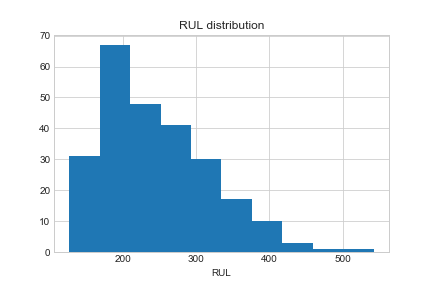
\includegraphics[width=0.6\textwidth]{plots/eda_rul_distribution.png}
    \caption{Training RUL distribution}
    \label{fig:rul-distribution}
\end{figure}

\begin{table}[!h]
    \centering
    \begin{tabular}{l|c}
        \hline 
        \hline \\[-1.8ex] 
        Statistic & Value \\
        \hline \\[-1.8ex] 
         N & 249 \\
         Mean & 244.98 \\
         Std. Dev. & 73.11 \\
         Min & 127 \\
         Max & 542 \\
         \hline
         \hline
    \end{tabular}
    \caption{Train RUL summary}
    \label{tab:rul-train-summary}
\end{table}

%%%%%% ---------------------------

\section{Preprocessing}\label{sec:preprocess}
Raw sensor data plotting reveals no clear patterns and insights about how each sensor trends over time until failure, as depicted in \autoref{fig:sensors-raw}. A visual inspection of the three operational settings variables indicates in [FIGURA OP SETTINGS] six different regions were samples agglomerate, which is expected given the six different operational regimes the engines can run. Back again to the raw sensor plotting over time, the intermittent behavior of the sensors measurement could be different operational regimes at each cycle - i.e., each operational mode shifts the operating range of each sensor and the operational conditions can be distinct at each cycle. Such hypothesis is supported by plots in \autoref{fig:rul-features-scatter-cluster}, where there are clear clusters for each sensor ranging from all possible RUL values, at least visually. Such scatter plots suggests that the operational condition can occur at any time of the engine, healthy or not, and changes intermittently. Clustering the series with kmeans algorithm, the clusters clearly emerge. 

Given that sensors operates at different ranges and, on top of that, operational conditions set new ranges for each sensor, the next logical step is to standardize each sensor to zero mean and unit variance according to the correspond operational regime. We have also removed features that are constant within at least one regime, since it would not add any new information to our model. The remaining standardized sensor charts are shown in \autoref{fig:sensors-std}, where is possible to see clear trends for some sensors over time. Sensors 1, 5, 16, 18 and 19 were removed since they were constant within at least one regime. Now it is clear that some sensors drift upwards and other downwards when the engines run towards failure. 

Additionally, since regimes seem to affect operating ranges, we added custom features to cumulative count the number of cycles each operational mode was run per unit.


\begin{figure}[!h]
    \centering
    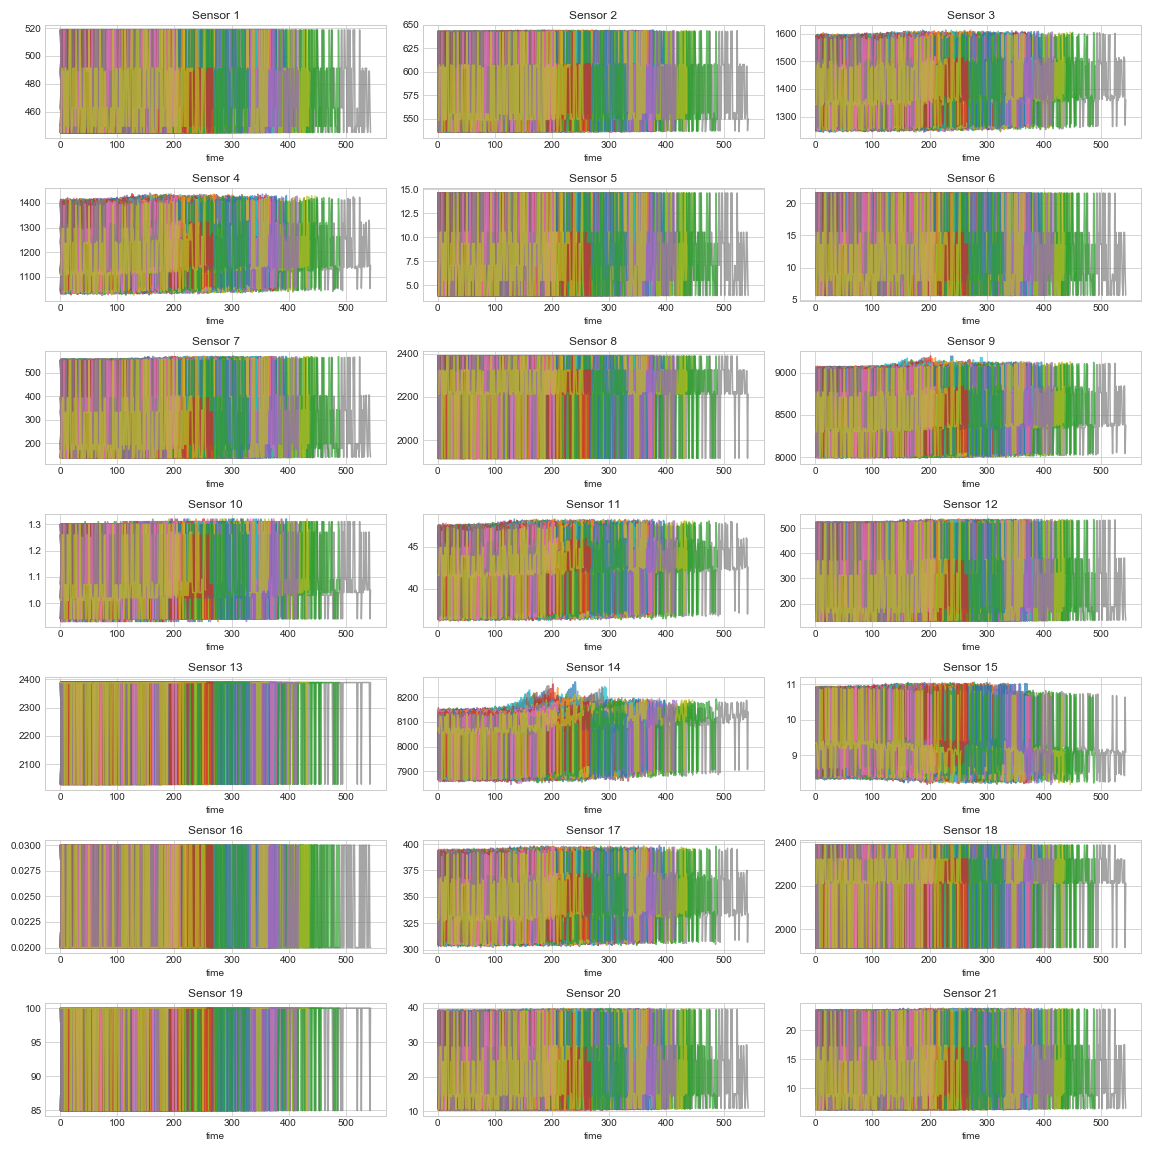
\includegraphics[width=0.9\textwidth]{plots/eda_sensors_raw.png}
    \caption{Sensor measurements raw data. Intermittent series with no clear trends emerging over time}
    \label{fig:sensors-raw}
\end{figure}

\begin{figure}[!h]
    \centering
    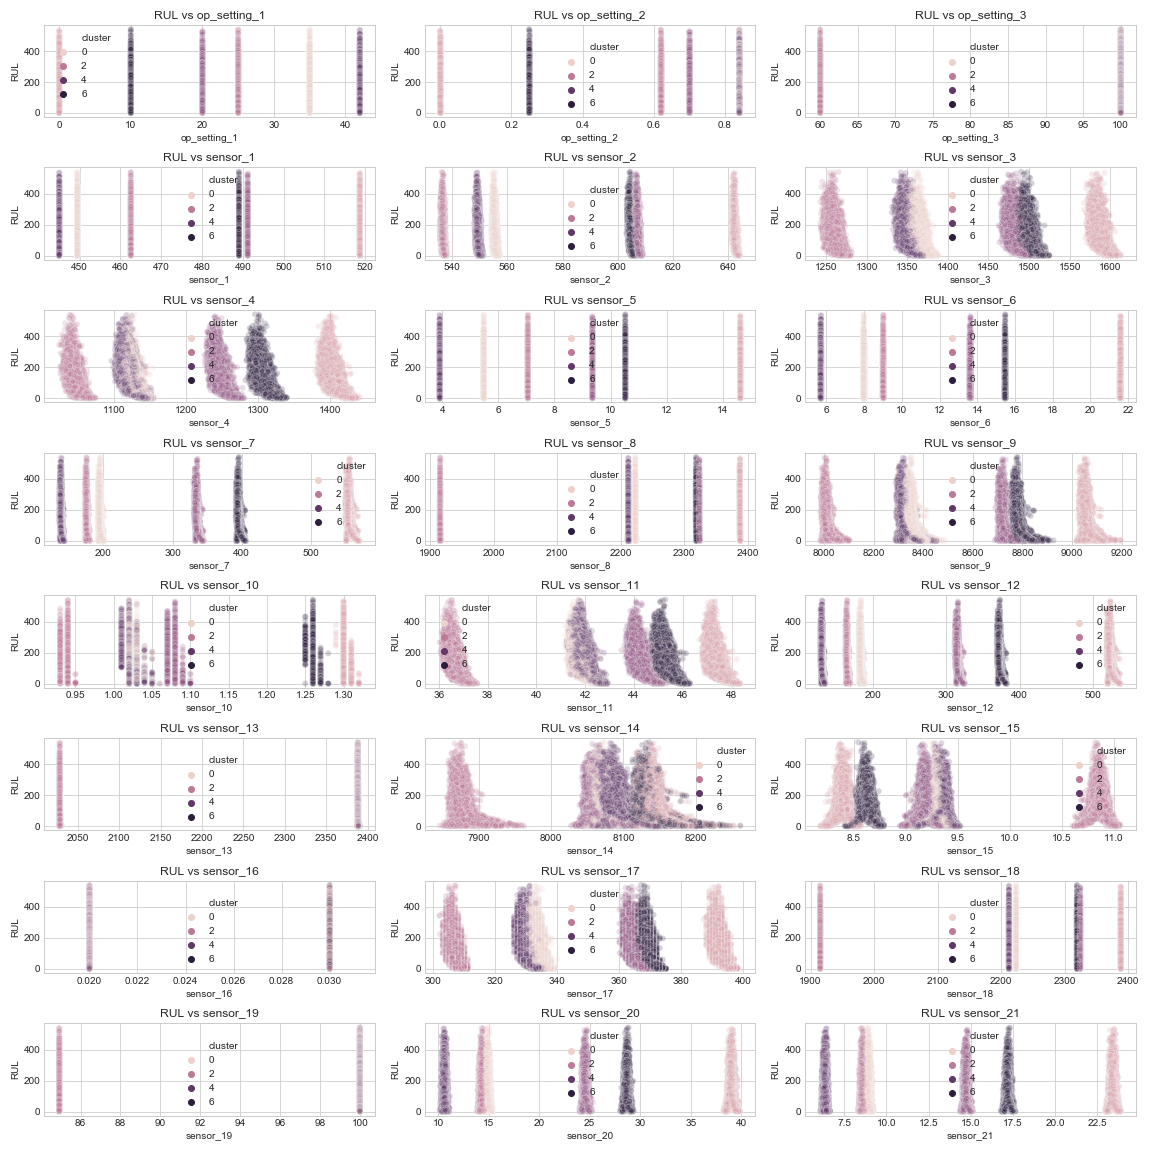
\includegraphics[width=0.9\textwidth]{plots/eda_scatters_cluster.png}
    \caption{RUL vs. each feature of the dataset. The six operational modes are clearly separable and identified by kmeans algorithm}
    \label{fig:rul-features-scatter-cluster}
\end{figure}

\begin{figure}[!h]
    \centering
    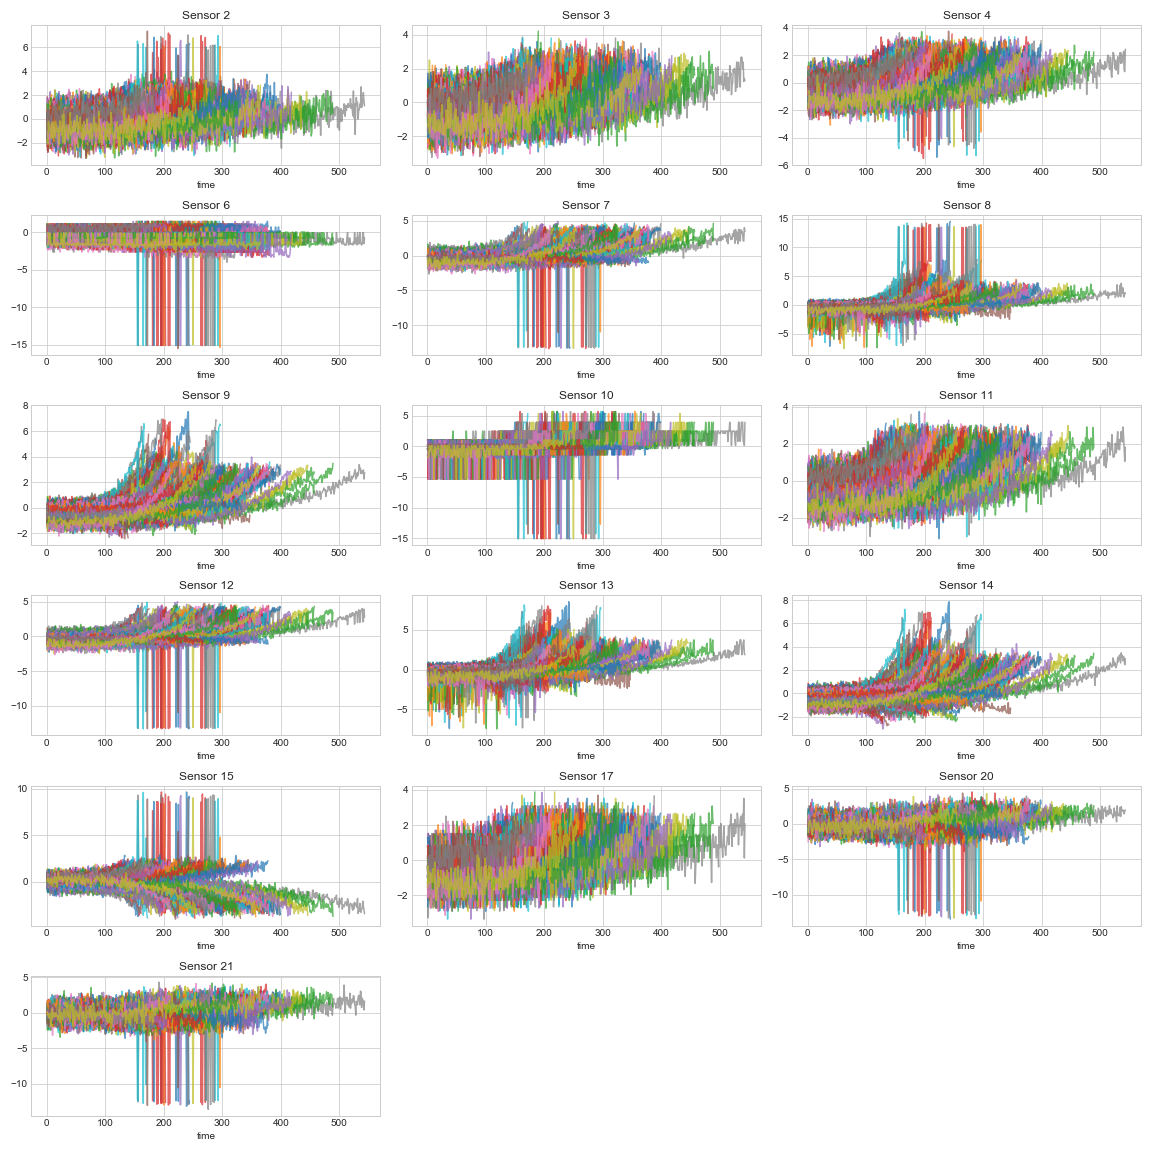
\includegraphics[width=0.9\textwidth]{plots/eda_sensors_std.png}
    \caption{Sensor measurements standardized for each regime. Now, clear trends over time emerges. Moreover, constant features within at least one regime were removed.}
    \label{fig:sensors-std}
\end{figure}

%%%%%% ---------------------------

\section{Modeling}\label{sec:modeling}
The formal derivations and construction of each algorithm used is out of the scope of this paper. For a more in-depth discussion about the underlying statistical assumptions for each model and applications, please refer to \cite{friedman2001elements}.

\subsection{Regression}
The idea behind using regression models is to generate a continuous output at any given input. Surely, with our data, the output, i.e. the RUL, is assumed discrete and the smallest step is one unit. Nevertheless, we did not postprocess our output to integer numbers.

The models selected here were: Linear Regression, Random Forest and Gradient Boosting. The first, linear regression, serve as a baseline model due its simplicity. However, one cannot underestimate the power of such simple model as we can give reliable, robust and, above all, interpretative estimations. Random Forest and Gradient Boosting are more complex models, that can also be used as classifiers as we did, that rely on ensemble of weak predictors. In addition, such models can capture non-linear relationships. They have tunable hyperparameter that are key to 

\subsection{Classification}
The classification task in RUL-related problems is usually set to classify answer whether the asset is at failure, unhealthy or operating at critical range. It is also possible to set the problem to predict if a failure will occur within a predefined horizon - and that is how we modelled and labelled our data. We encoded our target variable, RUL as:
\begin{equation}
	\operatorname{RUL}_\text{clf} = \begin{cases} 
		0, & \text{if RUL $\geq$ 20} \\
		1, & \text{if RUL $<$ 20}
		\end{cases} \; ,
\end{equation}
where the subscript $clf$ denotes the classification encoding.

Again, we used three models, being the simplest one, Logistic Regression, as baseline. Random Forest and Gradient Boosting, now as classifiers, were chosen for the same reasons of regression tasks.

%%%% ---------------------------

\section{Model Selection}\label{sec:model-selection}
\subsection{Evaluation Metrics}
We evaluate our predictions using two types of metrics: Mean Squared Error (MSE) for regression models; and $F_1$ score for classification.

The MSE is defined as:
\begin{equation}\label{eq:mse}
    \operatorname{MSE} = \frac{1}{N} \sum_{i=1}^{N} (y - \hat{y})^2,
\end{equation}
where $y$ is the true, or target, variable, i.e. RUL, $\hat{y}$ is the predicted RUL and $N$ is the sample size, i.e. the number of predictions. Such metric is symmetric, i.e. equally weights over and underestimations and penalizes greater deviations. Therefore, the smaller, the better.

The $F_1$ Score here is defined as the harmonic mean of \textit{precision} and \textit{recall}, a special case of the more general definition of $F_1$:
\begin{align}\label{eq:f1}
    F_1 &= \bigg( \frac{\text{precision}^{-1} + \text{recall}^{-1}}{2} \bigg) ^{-1} \nonumber\\
    &= 2 \cdot \frac{\text{precision} \cdot \text{recall}}{\text{precision} + \text{recall}} \; ,
\end{align}
where \textit{precision} is the true positive over positive predictions and \textit{recall} is the true positive over the true positive elements. Therefore, the greater, the better. In addition, it is clear that the possible values range from 0 to 1.

%%%%%% ---------------------------

\subsection{Cross-validation}
Cross-validation is widely used to evaluate machine learning algorithms performance. The main reason is to prevent overfitting, i.e. when the model cannot generalize predictions well to new unseen data.

The usual set up is to divide training data into folds, train the model in some and test on those left out and evaluate predictions using a metric. Then the process is repeated exhaustively to all possible combinations training and testing (or validation) folds. The mean score of all steps is usually used to compare algorithms. In this paper, we splited our data into 5 folds, each with approximatedly 50 engine units. We then left out one fold for validation and train the model on the other four.


%%%%%% ---------------------------

\subsection{Model selection}
Each regression and classification model selection is splitted into two parts. First, we cross-validate all three models and pick the best mean cross-validation score with the respective metric. Then, for the chosen model we fine tune its hyperparameters with grid search. Then, the best hyperparameter combination is is used to calibrate the model and then it is ready to be tested on the test set.

%%%%%% ---------------------------

\section{Postprocessing}\label{sec:postprocess}
For the chosen regression model, we post processed the predictions with Kalman filter \cite{h2oai}. It is not the scope of this paper to prove the underlying theory behind the filtering method - the reader can refer to \cite{kalman1960new}. 

The main motivation to use Kalman filter is to remove noisy predictions and to try to enforce that the next RUL value must be less than the previous, i.e. the RUL decreases by one unit after every cycle. It is possible to do that if a state space model of the system, where we can add prior knowledge (RUL decreases by 1 unit) and estimate the true state of the system given new information (the observations). In our case, our observations are our predictions.

The state space equations are give by
\begin{align}
	y_{t} &= \mathbf{G}\mathbf{x} + \nu_t \quad \text{where $\nu \sim N(0, \sigma^2)$} \\
	\mathbf{x}_{t+1} &= \mathbf{A}\mathbf{x}_{t+1}
\end{align}
where $y_t$ is the observation at time $t$ that is given by the observation model matrix $\mathbf{G}$ and it is noisy, by definition, through $\nu$. The state transition is given by the transition matrix $\mathbf{A}$ and it is, also, usually noisy, but here we assumed to be deterministic.

To keep it simple, we modelled with states $\mathbf{x} = [\operatorname{RUL}, -1]'$, transition matrix $\bigl[ \begin{smallmatrix}1&-1 \\ 0&1\end{smallmatrix} \bigr]$, and the variance $\sigma^2$ of the noise $\eta$ is given by the model $MSE$ The observation model is defined as $\mathbf{G} = [1, 0]`$. Therefore, with a little algebra, one can confirm that the $\operatorname{RUL}_{t+1} = \operatorname{RUL}_t{ - 1}$ and the observations $y_t$, i.e. our predictions, are given by true $RUL_t$ plus some noise whose variance is equal to the model error.

%%%%%% ---------------------------

\section{Results}\label{sec:results}
\subsection{Regression}
The training cross validation mean scores are shown in \autoref{tab:reg-train-scores}. Both complex models beat linear regression and the best performer was Gradient Boosting. The Random Forest was trained with 100 trees, no limit for max depth and minimum samples for spliting was 2. The Gradient Boosting model was trained with 100 estimators, learning rate of 0.1 and max depth of 3.

We proceeded with hyperparameters tuning for the best performer, Gradient Boosting, and the final model was set up with 100 estimators, learning rate of 0.03 and max depth of 5. The mean CV MSE score improved only 1\%, down to 2,714.60. After Kalman post processing, the results were improved by 20\%, down to MSE of 2,162.77. In \autoref{fig:test-preds-reg} it is possible to see how Kalman filters treated the signal for 4 random selected testing units.

The test scores were almost 2 times worse than training: 4,781.52 without filtering and 4,699.35 after filtering. The linear regression test score was 5,467.76. Such decreaset can be due to the fact that most predictions are more accurate when the RUL is smaller, i.e., the engine is approaching to failure. This can be explained by the fact that health engines oeprates always at a constant health range for each operating mode, meaning that sensor data will only have variation due to nois. When approaching to failure, variation is caused by other factors and the model, then, captures it. It is almost as we would try to predict a decreasing target function with a constant input. In \autoref{fig:rul-actual-pred} we can see such relationship between actual and predicted RUL and in \autoref{fig:test-rul-dist} we can see that testing RUL are widely distributed - i.e. there are as many healthy and unhealthy engines.

\begin{table}[!h]
    \centering
    \begin{tabular}{l|c}
        \hline 
        \hline \\[-1.8ex] 
        Model & Mean CV MSE \\
        \hline \\[-1.8ex] 
         Linear Regression & 3,318.97 \\
         Random Forest & 2,900.40 \\
         Gradient Boosting & 2,744.74 \\
         \hline
         \hline
    \end{tabular}
    \caption{Regression training scores}
    \label{tab:reg-train-scores}
\end{table}

\begin{figure}[!h]
    \centering
    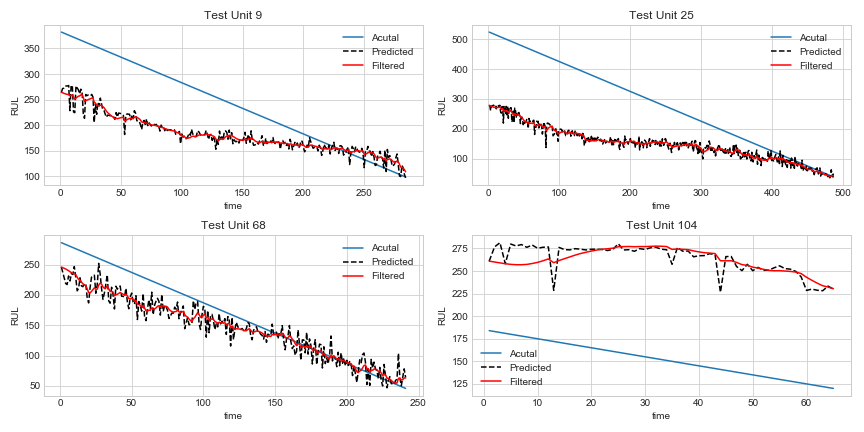
\includegraphics[width=0.9\textwidth]{plots/reg_test_units_pred.png}
    \caption{Random test units actual and predicted RUL, raw and postprocessed with Kalman filter}
    \label{fig:test-preds-reg}
\end{figure}

\begin{figure}[!h]
    \centering
    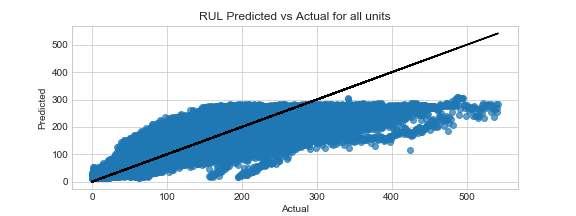
\includegraphics[width=0.9\textwidth]{plots/reg_rul_pred_true.png}
    \caption{Relationship between actual and predicted training RUL. There is a convergence when RUL approaches zero.}
    \label{fig:rul-actual-pred}
\end{figure}

\begin{figure}[!h]
    \centering
    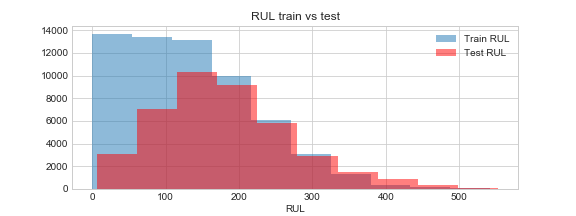
\includegraphics[width=0.9\textwidth]{plots/hist_rul_train_test.png}
    \caption{Test RUL are distributed accross a wide range}
    \label{fig:test-rul-dist}
\end{figure}

\subsection{Classification}
The training cross validation mean scores are shown in \autoref{tab:clf-train-scores}. Both complex models beat logistic regression and the best performer was Random Forest. The Random Forest was trained with 100 trees, no limit for max depth and minimum samples for spliting was 2. The Gradient Boosting model was trained with 100 estimators, learning rate of 0.1 and max depth of 3.

The test scores were almost 3 times worse than training: 0.52. Intereting the baseline model, logistic regression, had a better test score, 0.55. Again, noisy data and testing units that were not close to failure - and in this case below RUL of 20 - might affected the predictions and degraded performance.
\begin{table}[!h]
    \centering
    \begin{tabular}{l|c}
        \hline 
        \hline \\[-1.8ex] 
        Model & Mean CV $F_1$ \\
        \hline \\[-1.8ex] 
         Logistic Regression & .80 \\
         Random Forest & .84 \\
         Gradient Boosting & .83 \\
         \hline
         \hline
    \end{tabular}
    \caption{Classification training scores}
    \label{tab:clf-train-scores}
\end{table}

We proceeded with hyperparameters tuning for the best performer, Random Forest, and the final model was set up with 100 estimators and no limit for max depth of 10. The mean CV $F_1$ score decrease slightly to 0.83, but limiting the max depth is prefered in order to avoid overfitting. 


%%%%%% ---------------------------

\section{Conclusion}\label{sec:conclusion}
In short, our models performed well on training set, but, even though we have used cross-validation folds to avoid overfitting, it seems that they could not generalize well, since the test results were much worse. Perhaps a more thorough preprocessing improves model performance, with a more careful signal processing to remove noise.

A different target function, i.e. RUL, handling might help fix the fact that for healthy units the sensor data does not vary much except from noisy measurements. Therefore, an alternative approach is to create a healthy index and from it postprocess predictions with Kalman filtering taking into account transition matrix and the fact that RUL always decrease by one unit after each cycle.

%%%%%%%%%%%%%%%%%%%%%%%%%%%%%%%%%%%%%%%%%%%%%%%%%%%%%%%%%%%%%%%%%%%%%%%%%%%%%%%%
\newpage
\bibliographystyle{IEEEtranS}
\bibliography{references}

%%%%%%%%%%%%%%%%%%%%%%%%%%%%%%%%%%%%%%%%%%%%%%%%%%%%%%%%%%%%%%%%%%%%%%%%%%%%%%%%

\end{document}
